\section{Icelandic Turf Houses}

Turf houses are a significant part of culture and heritage in Iceland. A
paper published by Bathurst et al. \cite{ref01}, explains that turf has
always been widely used across regions in northern Europe for its
durability, renewability, and its abundance. It also has great
insulation properties which makes it a good choice for colder climates.
Since turf houses are unique, their appearance and construction garnered
a lot of attention and admiration from people. This leads to interesting
studies and research on their history, culture and construction
practices \cite{ref05}.

According to Lin et al. \cite{ref02}, regions such as Scotland and especially
Iceland have very limited supply of natural resources, however turf was
abundant. This made it very important for shelter construction. Turf
houses that were well built were also stated to be better in insulating
cold weather than houses built on stone and timber, which is very
important in these countries with harsh cold weather. Wunderlich et al.
\cite{ref03}, describes turf as a major component in buildings for Iceland
during the medieval period. The turf used in the construction of these
buildings was cut from local bogs or from edges of cultivated fields in
the area. For example, in Mosfellsbær, it was presumed that the bricks
of turf used were cut from the valley floor bogs, which was south of the
habitation area. The bogs were then transported to higher elevation
areas, where the difference in elevation naturally aided in draining
water, making it suitable for constructing houses \cite{ref01}.

Stone was often laid below the turf walls to prevent moisture from
seeping into the walls and eventually causing it to rot \cite{ref04}. The
amount of stone beneath the turf walls varied on use. For example, in
turf houses that sheltered animals, the stone layers were higher so that
it would prevent animals from damaging the turf by feeding on it or
rubbing against it. Archaeological studies suggest that in Iceland
specifically, the stone foundations were used less in buildings during
the Viking era when compared to later eras such as the Medieval and Post
Medieval \cite{ref03}.

Like any other natural resource with positive qualities, turf also has
its drawbacks. A book published by Nannini \cite{ref05}, explains that
insulation with turf was only tolerable since it was applied generously,
houses would have thick walls and almost completely no windows.
Additionally, settlers would burn dried manure inside these houses to
generate more heat. Combined with the lack of ventilation, this led to
very unhealthy environments. Another issue is that turf is
replenishable. This means settlers would have to renovate every few
years or so and force owners to refurbish or rebuild their home. Hannes
Larusson \cite{ref06} emphasizes this as ``an inseparable part of the turf
house'' which he later states as one of the main reasons why they were
eventually replaced by concrete.

With the innovation of concrete and the eventual abandonment of
refurbishing or maintaining these perishable turf houses, this led to
the loss and destruction of these historical buildings.

\section{Studies in Turf and Turf House
Maintenance}

Due to the unique architectural design of these turf houses, it became
one of the most researched topics on Icelandic architectural history.
Studies even dating back to the last decades of the nineteenth century
\cite{ref05}. Even today, many scholars and authors research on turf
construction from analysis of inner environment comfort to botany of the
turf layers \cite{ref07}. According to Sigurjón \cite{ref08}, many Icelandic
scholars and researchers such as architects, architectural historians
and conservation experts, have been extensively studying turf houses
solely focusing on restoring and conserving these sites.

Researchers such as Wunderlich et al. \cite{ref03}, conducted studies on
imaging medieval turf buildings in Iceland through geophysical methods.
This is to understand the structural features and subsurface
characteristics of the houses. During a study conducted by Milek and
Roberts \cite{ref09}, ash was discovered to be deposited on the floors of the
houses. This was used as insecticide and a drying material since the ash
can fill the tiny gaps and holes. It is also absorbent and hence can
protect the wooden materials from fungal decay. Studies from Milek
\cite{ref10} state that although turf buildings can last for over 100 years
when properly constructed and maintained, these buildings would still
need constant turf replacement. Specifically on the roof and walls,
since they are prone to rot. Stating that both turf and timber needs
replacement every 10 -- 20 years.

There has also been other research with goals specifically focused on
turf restoration in general. Studies conducted by Hnatowich et al.
\cite{ref11} have been transplanting healthy turf into disturbed areas with
hopes to restore it. By using native and local turf for the transplant,
there is an added benefit of lesser shock to the transplanted area.
Additionally, other studies such as those by Malleshaiah et al.
\cite{ref12}, have presented techniques such as soil aerification. This has
proved to improve turf quality by relieving the soil compaction, giving
it proper aeration and therefore improving turf quality. This is further
supported by Nunome et al. \cite{ref13} stating that soil compacting is a
major factor in the increase of degradation of turf.

With ongoing and continuous studies and discoveries on turf and turf
house construction and maintenance, preservation experts can further
study and utilize these techniques to extend the lifespan of these turf
houses. By minimizing rot and decay on these turf and wooden structures,
especially on the roof and walls, these turf houses can be properly
maintained while preserving the cultural heritage and importance of these
historical structures.

\section{LoRa Mesh Technology}

Long Range (LoRa) technology is a low-power wireless communication
technology used in applications such as traffic-light control, smart
street lighting, environmental monitoring, smart waste management,
energy management, and the Internet of Things (IoT)
\cite{tome2018longrange,enriko2023lorawan,zhu2019mesh,lozano2018smartwaste,andrade2019lora,andrade2023smartmeter}. Its long communication range and low
power consumption make it suitable for distributed monitoring systems.
Depending on the antenna, radio configuration, terrain, and deployment
environment, LoRa communication can reach several kilometres
\cite{centenaro2016longrange}. LoRa is therefore a suitable candidate for
low-bandwidth applications that require low cost and scalability
\cite{rahman2018lora}. Its potential has also been demonstrated in IoT
applications \cite{ayele2017lora}.

\begin{figure}[htbp]
\centering
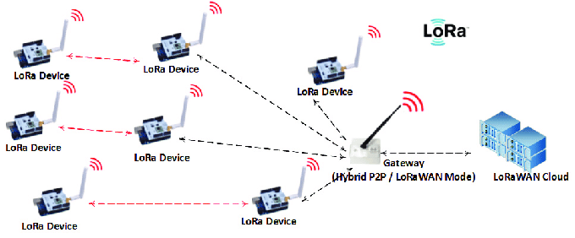
\includegraphics[width=0.8\textwidth]{figs/rrl-image1.png}
\caption{LoRa mesh technology illustrating multi-hop communication.}
\label{fig:rrl-image1}
\end{figure}

Multi-hop communication, mesh networking, and routing protocols can
extend the coverage and improve the signal reliability of LoRa networks
\cite{solar2022monitoring,sole2022mesh}. Mullick et al. reported improved
network performance when a mesh strategy was used for air-quality
monitoring, particularly under adverse environmental conditions
\cite{mullick2022mesh}. Andersen et al. also demonstrated that a LoRa mesh
network could approximately double the operating range of an asset-tracking
prototype through multi-hop communication and routing
\cite{andersen2020mesh}.

Multi-hop communication also introduces trade-offs. Although additional
hops can increase coverage, they may increase latency because nodes need
to coordinate transmissions and avoid collisions
\cite{centelles2021multihop}. This trade-off depends on the application:
some systems prioritize low latency, whereas remote environmental
monitoring systems may prioritize range, reliability, and low power
consumption. In addition, relay nodes can reduce the transmission distance
to the next node and may therefore improve energy efficiency
\cite{khonrang2022multihop}.

Compared with other low-power wireless technologies, LoRa is particularly
well suited to outdoor applications that require long range and low power.
Zigbee generally provides shorter-range communication, while NB-IoT can
provide broader cellular coverage and higher data rates at the cost of
greater dependence on cellular infrastructure and power consumption
\cite{liu2023zigbee,danladi2022lpwan}. The approximate ranges in
Table~\ref{tab:wireless-range-comparison} are indicative only and depend
strongly on the deployment environment and network configuration.

\begin{table}[htbp]
\centering
\caption{Approximate communication ranges of selected wireless technologies.}
\label{tab:wireless-range-comparison}
\begin{tabular}{lll}
\toprule
\textbf{Technology} & \textbf{Approximate range} & \textbf{Main dependency} \\
\midrule
Zigbee & 10--300 m & Local radio environment \\
LoRa & 2--15 km & Antenna, terrain, and radio settings \\
NB-IoT & Up to 100 km & Cellular network coverage \\
\bottomrule
\end{tabular}
\end{table}

\section{Low-Power Technology}

Wireless sensor networks require a reliable energy source for sensing,
processing, storage, and communication. Although some systems are powered
continuously from an outlet, remote monitoring nodes commonly rely on
batteries. For long-term deployments, reducing energy consumption is
essential because battery replacement may be difficult or disruptive.
Low-power design techniques can improve energy efficiency and extend the
operational lifetime of sensor nodes \cite{lahiri2002battery}.

One common technique is to place the device in a sleep state when it is
not actively sensing or communicating. During low-power operation, most
functions are disabled while a small control subsystem remains active to
restore normal operation when required \cite{zhang2023sleep}. For systems
with low duty cycles, the sleep period is often more important to overall
energy consumption than the active period \cite{hwang2012poweraware}.

Previous studies demonstrate the practical benefits of this approach.
Kombo et al. reduced the duty cycle of a low-power monitoring system to
less than one percent, while Hung et al. reported power-consumption
reductions of approximately 38.46--54.44\% using a low-power wireless
sensor protocol \cite{kombo2021groundwater,hung2020lowpower}. These results
support the use of scheduled sensing, selective peripheral activation, and
communication sleep modes in remote environmental monitoring.

Low-power operation is therefore central to the present system. The
proposed sensor nodes periodically wake, collect measurements, transmit or
store the data, and return to a sleep state. This duty-cycle strategy
reduces average current consumption while allowing the system to continue
monitoring environmental conditions over an extended deployment period.

\section{Cloud-Based Data Visualization and Management in Research}

Cloud-based data systems provide a convenient way to store, visualize, and
manage measurements collected by remote sensor networks. Researchers can
access time-series data without physically retrieving the sensor nodes,
which is particularly useful when monitoring sites are distant or difficult
to access. Cloud platforms also provide scalable infrastructure for storing
and processing large datasets \cite{naik2017cloud,sheffield2022cloud}.

Common cloud platforms include Amazon Web Services (AWS), Google Cloud
Platform (GCP), and Microsoft Azure. These platforms support different
combinations of data storage, analytics, visualization, and Internet of
Things services \cite{aws2023,gcp2023,azure2023}. The appropriate platform
depends on the required storage capacity, processing capability, cost,
connectivity, and ease of integration with the embedded system.

For environmental monitoring, cloud-based visualization can improve the
interpretation of long-term measurements by making trends and anomalies
available remotely. In the present project, cloud connectivity is used to
upload sensor measurements to ThingSpeak, where the data can be stored and
visualized for subsequent analysis.

\section{Measuring Soil Moisture}

Measuring soil moisture is one of the fundamental techniques when
studying soil conditions in environmental monitoring research. Over the
years, soil monitoring techniques have been continuously improved, and
new methods have been developed. However, these methods vary in their
principles and specific applications.

The standard method of measuring soil moisture is the Gravimetric
Method. To measure the soil moisture, researchers must get the
difference of the natural weight of soil to the same amount of soil but
dried. This is often achieved by placing the soil in an oven to remove
moisture \cite{ref24}. Starr and Paltineanu \cite{ref25} state this method as
very simple and highly accurate to such a degree that it is often used
as a calibration for other sensors or methods. It is even used to
validate data gathered from different studies \cite{ref26}\cite{ref27}. The
formula for calculating the soil moisture is defined by:

\begin{equation}
Soil\ Moisture\ Content\ (\%) = \frac{Weight\ of\ Wet\ Soil - Weight\ of\ Dry\ Soil}{Weight\ of\ Dry\ Soil}\ x\ 100
\label{eq:gravimetric-soil-moisture}
\end{equation}

However, this method has its downsides, although being very simple. It
is very time-consuming and destructive for the study area since it
involves unearthing soil and taking the time to dehydrate it in the
oven. This makes it unsuitable for long term studies and real time
monitoring \cite{ref24}.

New and modern techniques that are highly accurate, fast and
non-destructive are the Time Domain Reflectometry (TDR) and the
Frequency Domain Reflectometry (FDR). Because there is a significant
difference between the dielectric constants of dry soil and pure water,
modern tools can easily distinguish between the two \cite{ref28}. TDR works
by placing steel rods into the soil and then sending electrical signals
through them. The signal travels from one probe through the other by
traveling through the soil. The property of wet soil makes it return the
signal slower compared to dry soil. In turn, this helps the device
determine the humidity of the soil accurately \cite{ref19}\cite{ref29}.

FDR works similarly to TDR, but instead of measuring the time it takes
for the signal to move through the soil, FDR measures the frequency of
the electromagnetic waves when it travels \cite{ref28}. When the
electromagnetic waves travel through the soil, the frequency of the
signal changes based on the moisture. This helps researchers determine
the soil moisture accurately and precisely \cite{ref30}. Although these
methods are quick and accurate without having the need to be
destructive, devices like these are expensive and can cost up to
hundreds or even thousands of dollars based on the application \cite{ref19}.

Nowadays, there are newer types of sensors which can be used to measure
soil moisture without having the need to be expensive all while being
fairly accurate, quick, and non-destructive. These sensors include
resistance-based and capacitance-based types. Resistance-based sensors
measure soil moisture by placing probes into the soil, similar to the
methods mentioned earlier. However, instead of sending electrical
signals or waves, this method measures the soil\textquotesingle s
resistance. The resistance of the soil lowers when it has a high amount
of moisture and rises when it is dry \cite{ref31}\cite{ref32}. However, Koyunco
et al. \cite{ref28} states that this method is highly unreliable because
soil types can vary in resistance which leads to imprecise results.
Additionally, the probes are prone to corrosion which can lead to no
results at all.

Capacitive sensors work by measuring the capacitance across the sensor
electrode due to humidity when deploying a pulse voltage
\cite{ref33}\cite{ref34}. González-Turel et al. \cite{ref35} explain that because
the dielectric constant of water is higher than that of air or dry soil,
the moisture content affects the dielectric constant. This results in an
increase when the soil is wet, leading to a higher capacitance that can
be detected by the sensor. Researchers like Kulmány et al. \cite{ref36}
prefer these types of sensors because they provide accurate data while
being inexpensive and easy to install. Additionally, these sensors are
less prone to oxidation and damage because they do not require exposed
probes to touch the soil; their sealed design provides adequate
protection.

Among most methods and sensors used for determining soil moisture,
typically capacitive sensors are often preferred for their accuracy,
inexpensive price, and ease of installation while being able to provide
real time data. Each method, however, has its own strength and
limitations, which are considered during research making one more
suitable than the others, especially for specific conditions.
Ultimately, the choice of sensor and methods will depend on the specific
requirements and parameters in the study and the choice of the
researchers. It's important to evaluate these factors and select the one
that is most appropriate for the study.